\documentclass{article}
\usepackage[utf8]{inputenc}

% Page setup
\usepackage[a4paper,landscape,margin=2cm]{geometry}
\usepackage{amsmath}

% Typography
\usepackage[scaled]{helvet}
\let\familydefault\sfdefault

\usepackage[usenames,svgnames]{xcolor}
\usepackage{tikz,pgfplots}
\usetikzlibrary{positioning,arrows,intersections,calc}

\definecolor{colorfile}     {RGB}{ 79,142,209}
\definecolor{colorsummary}  {RGB}{143,232,186}
\definecolor{colortext}     {RGB}{ 29, 29, 27}

\begin{document}
\pagestyle{empty}
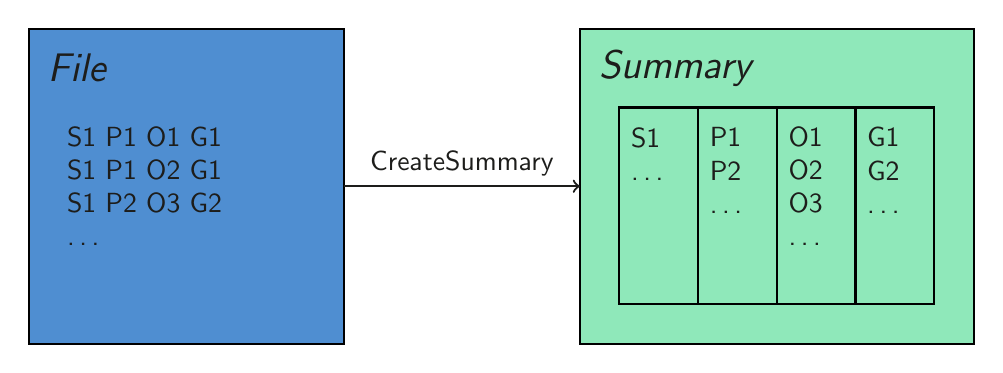
\begin{tikzpicture}[
    node distance = 10em, auto, thick,
    title/.style={text=colortext,font={\Large\itshape}},
    person/.style={text=colorwhite,font={\Large\bfseries}},
    code/.style={text=colortext,font={}},
    key/.style={text=colorkey,font={\tiny\itshape}}
]

    % File
    \draw[fill=colorfile] (0,4) rectangle (4,0);
    \node[title,text width=10em] at (2,3.5) {File};
    \node[code,text width=20em] at (4,2) {S1 P1 O1 G1\\S1 P1 O2 G1\\S1 P2 O3 G2\\\ldots};
    
    % Summary
    \draw[fill=colorsummary] (7,4) rectangle (12,0);
    \node[title,text width=10em] at (9, 3.5) {Summary};
    
    % Components
    \draw[fill=colorsummary] (7.5,3) rectangle (8.5,0.5);
    \node[code,text width=2em] at (8,2.4) {S1\\\ldots};
    \draw[fill=colorsummary] (8.5,3) rectangle (9.5,0.5);
    \node[code,text width=2em] at (9,2.2) {P1\\P2\\\ldots};
    \draw[fill=colorsummary] (9.5,3) rectangle (10.5,0.5);
    \node[code,text width=2em] at (10,2) {O1\\O2\\O3\\\ldots};
    \draw[fill=colorsummary] (10.5,3) rectangle (11.5,0.5);
    \node[code,text width=2em] at (11,2.2) {G1\\G2\\\ldots};

    % Arrows
    \draw[->,thick,colortext] (4,2) -- (7,2) node[midway] {CreateSummary};

\end{tikzpicture}
\end{document}
